%!TEX root = /Users/markelikalderon/Documents/Git/timaeus/timaeus.tex

\chapter{The Bonds of Life} % (fold)
\label{cha:the_bonds_of_life}

\section{The Soul--Body Union for Mortals} % (fold)
\label{sec:the_soul_body_union_in_mortals}

The soul-body union for mortals differs from the union of the World Soul and the body of the Cosmos. Mortal beings are not only embodied but embedded in an environment. The Cosmos may be an embodied living being, but it is not embedded in an environment, it is the environment. This is related to a further difference. Whereas the World Soul encompasses the body of the Cosmos, the bodies of mortal beings encompasses their soul. The soul of mortal beings is bound to their body and this bond must be protected from the effects of strong powers in the environment. Thus the Young Gods when weaving the immortal and mortal parts together position these bonds within. In this manner, the body encompasses the soul of a mortal being. The soul of mortal beings is bound to marrow, and this marrow is surrounded by hard bone to protect the bonds from external impact. Thus the skull is the primary fortification of the sovereign acropolis. By contrast, there are no strong powers external to the Cosmos that may age or weaken it. And hence no need of corporeal encompassment to protect what binds the World Soul to the body of the Cosmos. So the World Soul may, instead, safely encompass the body of the Cosmos. The souls of mortal beings are bound within since they are embedded in an environment with strong powers.

Two features of mortal anatomy are relevant to the soul-body union, the marrow and the bone that encases it. The marrow is not the bond of the soul but that to which the soul is bound. It has the character that it has for just this purpose. So Timaeus' account of the marrow will be informative about the soul-body union for mortals. The bone that encases the marrow is to protect the bond from the effects of strong powers in the environment. The soul of mortal beings has an immortal part and a mortal part. The immortal soul is bound to the marrow in the skull, called the ``brain''. The Young Gods made the skull spherical, in imitation of the shape of the Cosmos and the circular activity of cognition. The mortal soul is bound to marrow as well. Its roots are in the marrow of the spine. When contrasted with the circular skull, we are perhaps struck first by the linear character of the spine. But if we recall that the spine encompasses the marrow that it contains, we recognize that the spine is, more specifically, cylindrical. Recall that motions are either circular or linear. The skull takes its shape from the circular motion of cognition. The spine combines the circular and the linear in its shape. What may we infer about the mortal soul's bond with the marrow of the spine?

The linear aspect of its cylindrical shape is explicable given our previous discussion. Setting aside the possibility of cosmic perception (Proclus, \emph{In Timaeum} 2 83.3–85.31, \citealt{Diehl:1903re}, discussed in chapter~\ref{sec:knowledge_and_opinion}), \emph{aisthēsis} is a power of the mortal soul. \emph{Aisthēsis} involves a corporeal instrument that receives affections from strong powers in the perceiver's environment. Timaeus describes the action of these strong powers as linear. \emph{Aisthēsis} does not merely involve the reception of an affection from without, but importantly, it is the cognizance of the power of the agent that caused that affection. Perhaps the circular aspect of the spine's cylindrical shape reflects the circular activity that constitutes the soul's cognizance of the object of \emph{aisthēsis}. Later Platonists (such as Priscian, \emph{Metaphrasis in Theoprastum}, and Pseudo-Simplicius, \emph{In de anima}) will explicitly characterize perceptual apprehension as circular activity.

% section the_soul_body_union_in_mortals (end)

\section{Marrow} % (fold)
\label{sec:marrow}

God generated marrow from the finest elemental triangles. He chose only those elemental triangles that were unwarped and smooth. The triangles here, could not be the triangles of planar geometry \citep[293 n2]{Cornford:1935fk}. A warped triangle is not a planar figure. We have encountered this kind of issue before (chapter~\ref{sec:the_circles_of_the_same_and_the_different}). Thus, for example, the Demiurge formed two lines from the soul mixture and bent them back to form two circles. But a geometrical line cannot become a circle. The triangles should be understood on a material model. They are, after all, composed of sensible powers, traces of the Forms in the Receptacle, upon which the Demiurge has imposed form and number. In choosing only the finest elemental triangles, God ensures that they could exactly compose the purest fire, water, air, and earth. (I am uncertain why Timaeus departs, here, from the more usual ordering of fire, air, water, and earth.) God separated these triangles into kinds (presumably their shape) and mixed them in proportions that Timaeus does not reveal (perhaps for fear of impiety). He then fashioned the marrow from this mixture which Timaeus describes as the seed of all mortal kind. 

It is unclear what Timaeus means by this last remark. It is worth pausing over since talk of seeds and associated agrarian imagery predominates in Timaeus' account of marrow. It would be good to know in what sense marrow is a seed since Timaeus goes on to describe marrow as field that receives a divine seed. So is the marrow a seed or a seed bed? And in what sense or senses?

Later (91b1) Timaeus claims that marrow is the source of semen. So the marrow is the seed of all mortal kind since it is at the very least the source of the semen from which subsequent generations of mortals will spring. Notice, as well, the generality of Timaeus. Marrow is not merely the seed of human kind \citep[73]{Waterfield:2008lx} but of mortal kind. This encourages \citet[295]{Cornford:1935fk} to claim that ``the marrow is the fundamental life-substance in all animals and the same substance in all''. As we shall see, that marrow is described as universal seed since it is the fount of semen in mortals is not inconsistent with Timaeus subsequently describing marrow as a field or seed bed.

Though Timaeus speaks of the God in the singular here, the generation of the marrow is clearly a task that the Demiurge assigned to the Young Gods. The Young Gods, in generating the mortal parts, imitate the Demiurge's generation of the immortal part. Here, particulary, the \emph{mimēsis} is striking. The Demiurge generates the immortal soul by taking indivisible and divisible Being, Sameness, and Difference, mixing these, and using this mixture to fashion the immortal soul. Similarly, God generates marrow by selecting its components, mixing them, and fashioning the marrow. God's procedure is the corporeal analogue of the Demiurge's generation of the incorporeal soul.

God implanted in the marrow various kinds of soul. Allow me to make two sets of remarks about this deceptively simple claim.

First, \emph{Phuteuō} can mean implant, beget or engender, or to produce or bring about more generally. I translate (with \citealt[271]{Archer-Hind:1888qd}, \citealt[293]{Cornford:1935fk}, \citealt[70]{Lee:2008ca}, \citealt[77]{Taylor:1929ov} \citealt[73]{Waterfield:2003gs}, and \citealt[67]{Zeyl:2000cs}) \emph{phuteuōn} as implanted. Even if \emph{phuteuōn} could mean engendered in this context (as \citealt[191--3]{Bury:1929jb} translates), given the prominence of the agrarian imagery, the association of implanting carried by the Greek is salient. Recall that the immortal soul, in its celestial descent was sown in the instruments of time, and this signaled a greater involvement in corporeality than when it was merely a passenger in a stellar vehicle (chapter~\ref{sec:the_laws_of_destiny}). When it is implanted in the marrow that involvement is greater still for it is now embodied and embedded in an environment with strong powers.

Second, God implants in the marrow various kinds of soul. What kinds of soul does Timaeus have in mind? There are two alternatives. The kinds in question may simply be the immortal and mortal kinds. Or, given that the mortal soul has spirited and appetitive parts, the kinds may be reason, spirit, and appetite. On the first alternative there are two kinds on the second there are three. This may not seem like much of a difference given that the second kind of the first alternative, the mortal soul, divides exhaustively into the second and third kinds of the second alternative, spirit and appetite. But indifference between these alternatives betrays an insensitivity to a substantive explanatory difference. Are there two fundamentally different kinds of soul or three? Cast in these terms, it would seem that there are two, the immortal and mortal kind. The former does not perish upon death though the later does (though later Platonists envision the possibility of life after death for even the mortal soul, to animate the powers of shades in Hades, say). The Demiurge generates the immortal soul. The Young Gods generate the mortal soul. For recall, the Demiurge is incapable of generating anything mortal. And while spirit and appetite differ in their powers, locations and corporeal instruments, there does not seem to be a fundamental difference between them the way there is between sovereign reason and the broader \emph{polis}. This was manifest in the political toplogy of the soul. Reason occupies the acropolis, raised on a hill, surrounded by water and joined to the mainland and the broader \emph{polis} by a narrow isthmus. The social distance between the occupants of the acropolis and the occupants of the broader \emph{polis} is manifest in their spatial distance. And the splendor and fortification of the acropolis emphasize this. 

Having implanted the various kinds of soul in the marrow, God now divides that marrow. The divisions of the marrow correspond to the number and shape of the kinds of the souls implanted there. Again, this is a deceptively simple claim.

First, note the oddity of God's procedure. The kinds of soul are first implanted in the marrow and then the marrow is separated and formed into shapes that match the kinds. One might have expected, instead, that the marrow was divided and shaped first and then the various kinds of souls implanted in the appropriate divisions of marrow. Why does God proceed otherwise? Given His intellect and benevolence, it must be for the best. Perhaps God implants the various kinds of soul in undivided marrow because of the unity of the souls of mortal beings. It is one thing for Timaeus to distinguish parts of the soul. It is another to maintain that there are distinct rational, spirited, and appetitive souls. Even reason persisting when spirit and appetite perish, does not, by itself, establish this. Perhaps, then, God's implanting soul in undivided marrow dramatically emphasizes the unity of the soul of mortal beings (though, of course, questions remain).

Second, the number and kinds of shapes of the divided marrow correspond with the number and kinds of shapes of the souls implanted there. What is the number of souls? If the number of souls is one in each case there is not much point in making number explicit. This really only makes sense if the number could be more than one. So, for example, we know that there is only one part of the soul implanted in the head, the immortal part. What about the mortal part? The mortal part itself divides into spirit and appetite. if there are separate divisions of marrow for spirit and appetite, then the number in each case is one. But that is the trivial case. But if the mortal soul is implanted in its own marrow, then the number of souls (strictly parts of soul) implanted there are two. Thus the fundamental division of the soul into the immortal and mortal part is preserved, consistent with the further subdivision of the mortal soul required for tripartition.

Third, Timaeus' language here remains neutral concerning an important topic. What is the relationship between the shape of the marrow and the shape of the soul implanted there? If the soul is extended, then perhaps the marrow must be so shaped otherwise the soul would not fit. Or, if the soul is inextended, perhaps the shape of the marrow is modeled on an inextended paradigm. Timaeus does not specify the explanatory relationship, such as efficient causation or paradigmatic causation, if any, between the shape of the marrow and the shape of the soul implanted in it. Timaeus merely claims that they match.

God first divides the marrow that receives the immortal soul. This He makes into a sphere. Since the sphere of marrow received the immortal soul, and given its divine nature, Timaeus likens the marrow to a plough-field receiving divine seed. God calls this sphere of marrow ``brain'' (\emph{engkephalon}).

First, while Timaeus remains silent on the explanatory relationship between the shape of the soul and the shape of the marrow, details of the narrative would seem to rule out one natural alternative. Notice that the kind of soul---strictly, a part of a unified soul---is implanted in the undivided marrow. The marrow is then divided. And only then is it shaped into a sphere. That means that the immortal soul was implanted in the marrow before it was spherical. If that is right, then it is not the case that the marrow has its shape so that the relevant kind of soul will fit. The immortal soul fit fine when implanted in the undivided marrow.

Second, the agrarian imagery continues. The soul, and not the marrow, is now portrayed as a divine seed. The immortal soul is divine. It can apprehend in understanding divine intelligible things, and so assimilate to them. Timaeus has already described the soul as sown in the instruments of time and subsequently implanted in the undivided marrow. Since seeds are what one plants, this is a natural elaboration of the agrarian imagery. But it is an elaboration. Timaeus highlights the way in which seeds contain within themselves the power of growth and vital activity. Perhaps, the immortal soul is the divine seed since it is a divine principle of vital activity embedded within corporeal material designed to receive it. The marrow, of course, in being generated from the finest elemental triangles in the right proportions, was divinely prepared to receive the divine seed and so is likened to a plough field.

Describing the soul as divine seed implanted in the field of marrow is consistent with Timaeus' earlier description of marrow as universal seed. Indeed, the descriptions may be complementary. The marrow is like a field since it receives the divine seed and this activates vital activity in the newly incarnate mortal. The marrow is itself universal seed since it is the fount of semen. But as this is vital activity, the marrow is only the fount of semen insofar as the divine seed has been implanted there by God.

Third, a name is bestowed upon this spherical division of marrow. God calls it ``brain''  (\emph{engkephalon}). As \citet[77 n2]{Taylor:1929ov} and \citet[293 n3]{Cornford:1935fk} observe, this is most likely derived from \emph{en kephalē}, in the head. Given its gross observable features, it is perhaps natural to first regard the brain as the marrow of the skull. Timaeus claims that every living thing has the head as the container for the brain.

If the immortal soul is assigned to one division of marrow, the mortal soul is assigned to a plurality of divisions of marrow. God forms these into shapes that were both circular and linear. They have cylindrical shapes. Think, for example, of the shape of the marrow in the femur, or a bone in a finger. Upon these God bestowed the name ``marrow''.

The marrow is a divided seed bed. Nevertheless, from these, as from anchors, God bound the whole soul.

First, concerning the plural reference of ``these'', I take Timaeus to mean not only what God calls ``marrow'' but also what God calls ``brain''. For what is bound is the whole soul. And the whole soul includes the immortal part implanted in the brain.

Second, Timaeus shifts from agrarian to nautical imagery. The divided marrow anchors the whole soul. If the marrow is an anchor, then the soul is a ship tethered to this anchor by ropes or chains. The buoyancy of a ship keeps it afloat and so up from the floor of the sea. The image suggests that the corporeal is weighing down the whole soul which, if left to its own devices, might move upward in a celestial ascent (as in the \emph{Phaedrus} myth).

Third, Timaeus is unfortunately reticent about the nature of the bonds that anchor the whole soul to the divided marrow. Whatever their nature, they must be so as to bind the incorporeal to the corporeal. If we think of corporeal bonds such as ropes and chains this can seem puzzling. But not all bonds are corporeal. Timaeus, for example, claims that proportion is a bond, but proportion is not a body. Moreover, we have seen how this incorporeal bond may bind the corporeal. The Empedoclean ``roots'' are bound together by proportion in the body of the Cosmos. Timaeus does not say that the bonds that anchor the whole soul in the divided marrow are proportions. Nevertheless, what reflection on proportions as bonds reveals is that there is room within Timaeus' framework for a bond that binds the corporeal and the incorporeal.

We are now in a position to observe that Timaeus has posited three kinds of bonds, with the bonds that anchor the whole soul to the divided marrow being an intermediary kind. Let us consider the extremes first. On one extreme, there are incorporeal bonds that can only be undone by the agent that bound them. Examples of these are the proportional bonds that bind the primary bodies of the Cosmos  (32c3--5, chapter~\ref{sec:the_elemental_composition_of_the_corporeal}), the Young Gods (41a7--b6, chapter~\ref{sec:the_demiurge_addressing_the_gods}), the immortal part of the soul (43d, chapter~\ref{sec:the_shock_of_embodiment}), and the opposed extremes of white and black (68c7–d7, chapter~\ref{sec:the_eyes}). On the other extreme, there are corporeal bonds that can be undone even by agents other than the one that bound them. The invisible rivets with which the Young Gods bind the mortal parts (43a3–6, chapter~\ref{sec:the_shock_of_embodiment}) is an example of this. The bonds that anchor the whole soul to the divided marrow seem to be an intermediary bond that shares features with each of the opposed extremes. While the bonds that anchor the soul are most likely incorporeal, like corporeal bonds, they may be undone by agents other than the one who bound them, thus making the fortification of the acropolis necessary.

% section marrow (end)

\section{Bone} % (fold)
\label{sec:bone}

The whole soul is anchored to the divided marrow, and around this God constructed a shelter from a framework of bone. Bone is the primary fortification of the acropolis.

Timaeus begins by describing the generation of bone. He evidently takes his lead from Empedocles but offers a modification of that account. According to Empedocles:
\begin{verse}
	And pleasant earth in her well-built channels (\emph{choanoisi})\\
	received two parts of gleaming Nestis out of eight\\
	and four of Hephaistos; and they become white bones\\
	fitted together with the divine glues of harmony.\\
	(Empedocles, DK 31B96; \citealt[62 245]{Inwood:2001ve})
\end{verse}
Nestis is a Sicilian water goddess, and Hephaistos is associated with fire. Thus on a straightforward reading of the fragment, bone is generated by combining four parts fire with two parts earth and two parts water. (Though some commentators take Nestis to refer to water and air, perhaps under the influence of the general conviction that all four ``roots'' are present in every compound body, \citealt[209 n2]{Wright:1981zr}.) 

\citet[301-2]{Palmer:2009qf} maintains, however, that the straightforward reading of the fragment is flat footed. Specifically, he maintains that (\emph{choanoisi}) should not be translated as channels or hollows (as \citealt[151 n1]{Guthrie:1965ys}, \citealt[208--9]{Wright:1981zr}, \citealt[62 245]{Inwood:2001ve} do), but rather as a crucible. Hephaistos' involvement in the fragment makes this reading salient. So understood, Empedocles is not merely putting forward a list of ingredients from which bones may be mixed but a recipe for the generation of bone. Specifically, earth is first transformed into mud with the addition of water, and then this mixture is hardened by being fired in the crucible.

Timaeus would seem to accept a similar interpretation, for his account of the generation of bone further elaborates upon the metallurgic imagery. Moreover, Timaeus is similarly offering a recipe, a description of the process by which bone is generated. At the very least, Timaeus seems to regard this kind of interpretation as independently defensible, regardless of whether Empedocles subscribes to it. Perhaps this licenses the departures Timaeus makes from Empedocles' account. 

According to Timaeus, the procedure for generating bone consists of three steps:
\begin{enumerate}[(1)]
	\item God selects only earth that is smooth and pure by filtering it
	\item God mixes the selected earth with marrow
	\item God places the compound first in fire, then water, repeatedly
\end{enumerate}
Let us consider these in turn.

(1) \emph{God selects only earth that is smooth and pure by filtering it}. There is precedent for this in God's selection of the triangles that compose marrow. Only the finest triangles, unwarped and smooth, were chosen. Concerning the material that will fortify the acropolis, God is similarly selective. However, He begins not with elemental triangles, but with the primary body, earth. This perhaps explains the difference between the criteria for selection. Earth may be smooth, like the triangles that compose marrow, but no mention is made about being unwarped. The relevant sense of unwarped, I take it, is applicable to the elemental triangles and not to the bodies that may be composed of such triangles. Presumably the smoothness of earth consists in the cubes that compose it being small and relatively uniform in size. God selects only the finest earth. Not only is God selecting for the smoothness of earth but also its purity. So any other primary bodies, such as air or water, are filtered out and perhaps any unattached elemental triangles as well. The selection is described as a kind of filtering or sifting, and so we may imagine the craftsman God filtering earth through a sieve that selects only sufficiently small cubes of earth.

(2) \emph{God mixes the selected earth with marrow}. The first step was an elaboration of the Empeoclean account insofar as Empedocles makes no mention of the divine selection of earth. If the first step of the procedure is, in this way, an elaboration, the second step is a more significant departure. According to Empedocles, earth and water are mixed and so form the substantial mixture from which bone is generated. This is true both on Palmer's \citeyearpar{Palmer:2009qf} interpretation and the more straightforward alternative. The only difference is that, on the latter, more besides goes into the substantial mixture. However, water is no part of the substantial mixture but is used, instead, to treat that mixture in the process of bone generation. Timaeus substitutes a secondary body, marrow, for this primary body, water, to mix with earth. However, marrow is understood to be moist in the way that water is. And so presumably the resulting compound is muddy if not strictly speaking mud.

Why substitute marrow for water? Timaeus does no explicitly say. Consider, however, the following two suggestions.

First, perhaps we are meant to imagine that the result of this procedure is a compound of bone and marrow with hard bone on the outside and soft marrow within. Perhaps the moist marrow is dusted in earth that binds to it. Repeatedly firing and watering down the compound results in soft marrow surround by hard bone. I have my doubts. First, we depart from Empedocles where, on any interpretation, earth is mixed with water. If the Empedoclean parallel is to be maintained, then earth would be mixed with moist marrow. But it is not. On the present suggestion, earth merely dusts the moist outer surface of the marrow and binds to it. Another problem concerns the further fabrication that bone undergoes. Thus God fabricates the spherical skull on a lathe---a hazardous procedure, if the marrow remains within.

For these reasons I favor the second, admittedly speculative, suggestion. Perhaps generating bone from a substantial mixture that includes marrow guarantees that bone has some affinity for marrow. If so, that only raises the further question, why should the fortification of the acropolis share an affinity with its occupant? Consider the following speculative reason. Bone must be hard in order to protect the the divine bonds of life anchoring the whole soul to the divided marrow within from external impact. Perhaps bone, in being composed, in part, of marrow, retains an affinity with marrow and this functions to lesson the effect of any external impact upon the marrow. Thus when an external blow impacts upon the head, the hardness of the skull may prevent the marrow from being directly impacted, but the marrow will move within that hard skull and suffer a secondary impact against it. But suppose the skull, though hard, has an affinity with marrow. This will mean that it is less likely for the skull to act upon the marrow upon the secondary impact. After all, like does not act upon like. Having marrow as part of the substantial mixture of bone would thus function analogously to padding within a helmet (see figure~\ref{fig:helmet}).

\begin{figure}[htbp]
	\centering
		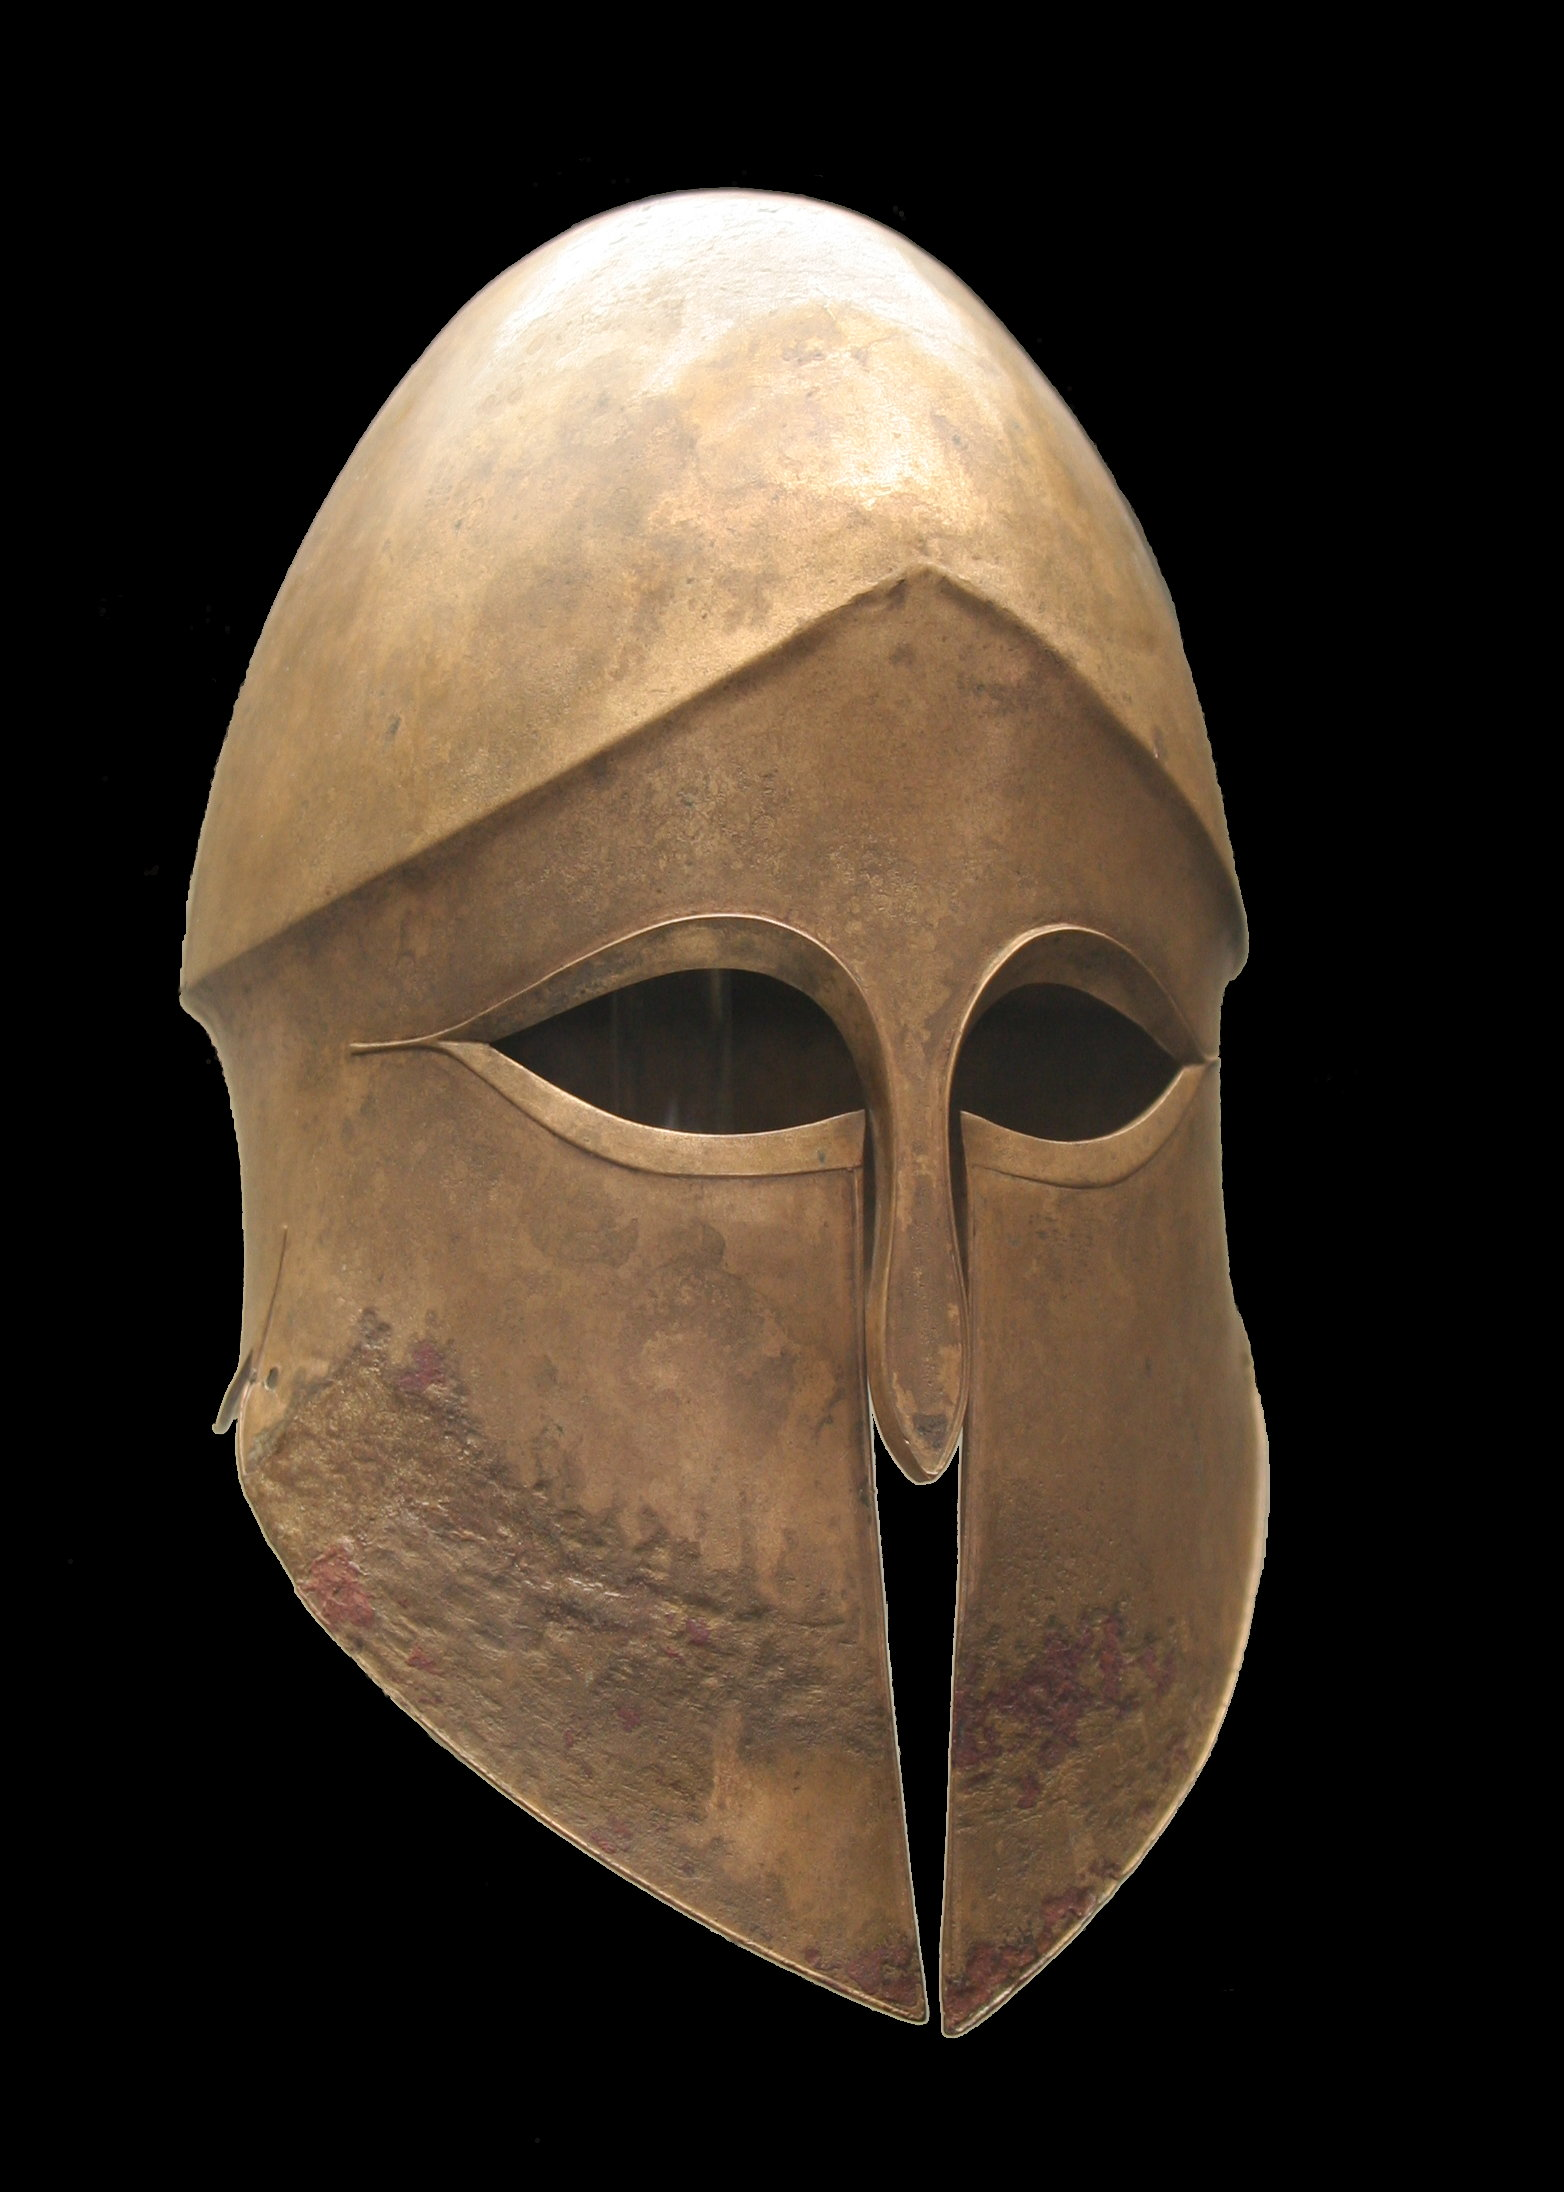
\includegraphics[scale=0.1]{graphics/helmet.jpg}
	\caption{Bronze Corinthian helmet, ca 500 BCE, Staatliche Antikensammlungen}
	\label{fig:helmet}
\end{figure}

(3) \emph{God places the compound first in fire, then water, repeatedly}. We have already observed that Timaeus replaces water with marrow in the substantial mixture from which bone is generated. Water plays role in the procedure for generating bone but not as a part of the substantial mixture. Instead, Timaeus assigns water a distinct role in his further elaboration of the metallurgic imagery. God takes the compound, the substantial mixture of earth and marrow, and fires it. He then cools it by plunging the compound in water. These two steps, firing and watering, are repeated many times. The metallurgic imagery here is vivid, especially if we bear in mind Hephaistos' involvement in the Empedoclean account. We are clearly meant to imagine a blacksmith pulling an iron out of the fire and cooling it by plunging it into water. Nevertheless, Timaeus' rationale for this procedure is not metallurgic. God exposes the compound to fire and water so that it may not be soluble by either primary body. Notice that there is no explicit mention here of hardening. Though since we began with a muddy mixture of fine earth and moist marrow, a soft compound, unlike the hard bone that is generated from repeatedly firing and watering it, it is safe to say that that the compound is also hardened in this process. The metallurgic imagery encourages this. And it is appropriate that hard bone be produced in a divine forge, like Hephaistos', since it is the fortification of the marrow, and among the things forged by a blacksmith is, importantly, armor. This is confirmed later in Timaeus' discussion of sinews where he claims that increasing the number of firings and waterings increases the hardness and inflexibility of bone (74b).

The procedure for the generation of bone results in boney stuff from which bones are themselves fabricated. The relevant craft seems to shift from metallurgy to carpentry. Thus, for example, the craftsman God seems to fabricate the skull on a lathe. Timaeus describes the fabrication of the skull and the vertebrae that compose the spine. These are not the only bones recognized by Timaeus. Timaeus singles out these two classes of bones given their special status. All bones contain marrow. And all marrow contains soul. But not all marrow contains enough soul for intelligence. The skull contains sufficient marrow to be the seat of intelligence. If the immortal part of the soul is anchored to the marrow of the skull, then we shall see that the mortal part of the soul is anchored, primarily, to the marrow in the spine.

The spherical skull is fabricated by spinning it. Clearly the craftsman God fashioned the spherical skull on a lathe. It is unclear, though, how the spherical skull comes to encompass the brain. The alternative reading, where marrow is not part of the substantial mixture from which bone is formed but is rather dusted with earth that binds to it, admittedly faces no such difficult. It has the advantage that the soft marrow is baked in, and only the earth-dusted surface is hardened into bone around it. This is a neat solution to our present difficulty. But, again, it fails to parallel Empedocles in not making marrow a part of the substantial mixture, and it is hard to square with fashioning the skull on a lathe, which would be a procedure fraught with danger if possible at all.

After fabricating the skull, God fabricates the vertebrae that compose the spine. Like the skull, vertebrae are composed of hard bone and encompass marrow that anchors a great amount of soul. There are, however, a number of striking contrasts:
\begin{enumerate}[(1)]
	\item While the skull is one, the vertebrae that compose the spine are many
	\item While the skull is circular, the spine is linear, the vertebrae that compose the spine being vertically stacked
	\item While the skull is inflexible, the spine is flexible since there are pivots between the vertebrae.
\end{enumerate}
Let us consider these differences in turn.

(1) \emph{While the skull is one, the vertebrae that compose the spine are many}. This may be a corporeal echo of the structure of the soul. Recall, the Circle of the Same is sovereign in that it governs the revolution of the Circle of the Different. And since it is sovereign, the Demiurge allows it to be undivided unlike the Circle of the Different. The skull is the primary fortification of the acropolis in which the immortal soul is anchored. The immortal soul has sovereignty over the mortal soul and the body that it animates. Presumably for this reason, its primary fortification consists in the unitary skull. The mortal soul, by contrast, is anchored in the spine. As it is governed, like the Circle of the Different, it is not exempt from division.

(2) \emph{While the skull is circular, the spine is linear, the vertebrae that compose the spine being vertically stacked}. The skull is a sphere made in imitation of the shape of the Cosmos. The spine, however, is linear, being composed of vertically stacked vertebrae. This manifests a difference in cognitive power, broadly conceived. Whereas the immortal soul anchored in the brain encased within the skull engages in the circular activity of cognition, the mortal soul, anchored in the marrow of the spine is subject to linear \emph{aisthēsis}. \emph{Aisthēsis} arises from the affection of the perceiver's body, when the parts affected are surrounded by mobile parts so that the affection may reach the soul. And the activity of the power that caused this affections is linear. Thus the fortification of the marrow that anchors the mortal soul reflects, in its shape, the power of \emph{aisthēsis}, just as the fortification of the acropolis reflects, in its shape, the power of cognition.

While the spine is linear, it encompasses the marrow with its stony substance. So, as we observed before, its overall shape is that of a cylinder. The linear aspect of the cylinder may reflect the linear nature of \emph{aisthēsis}, but its circular aspect may reflect the power to apprehend the objects of perception.

(3) \emph{While the skull is inflexible, the spine is flexible since there are pivots between the vertebrae.} This third difference is related to the first. The spine is compound, being composed of a plurality of rigid parts, the individual vertebrae, joined together with pivots. Given its plurality and the nature of its construction, the spine, as a whole, is flexible in the way that the skull, as a whole, is not. And again this may be a corporeal echo of the structure of the Soul. Compare how the divisions in the Circle of the Different in the World Soul is manifest and makes possible the complex motions of the wanderers. Similarly the divisions in the spine is manifest and makes possible the flexible movement of the spine. 

% section bone (end)


\section{The Location of the Mortal Soul} % (fold)
\label{sec:the_location_of_the_mortal_soul}



% section the_location_of_the_mortal_soul (end)

\section{The Unity of the Soul} % (fold)
\label{sec:the_unity_of_the_soul}

% section the_unity_of_the_soul (end)

% Chapter the_bonds_of_life (end) 